% LaTeX file for a 1 page document
\documentclass[a4paper, 11pt]{article}
\usepackage[utf8]{inputenc}
\usepackage[T1]{fontenc}
%\usepackage[ngerman,english]{babel}

\usepackage{amsmath}
\usepackage{commath}
\usepackage{textcomp}
\usepackage[squaren,thinspace,thinqspace]{SIunits}
\usepackage[minionint, lf]{MinionPro}
\usepackage[medfamily, sansmath, lf]{MyriadPro}
\usepackage[usenames,dvipsnames]{xcolor}
\usepackage{soul}

\usepackage{tikz}
\usetikzlibrary{arrows,shapes,positioning,shadows,trees}

\usepackage{microtype}
\usepackage{graphicx}
\usepackage{lipsum}
%\usepackage[normalem]{ulem}
\usepackage[round]{natbib}
%\usepackage{url}
\usepackage{titlesec}
\usepackage{geometry}
\usepackage{verbments}
%\usepackage{minted}
\usepackage{multicol}
\usepackage[font=small,labelfont=bf]{caption}
\usepackage{subcaption}
\usepackage{booktabs}
\usepackage[title]{appendix}

\usepackage{pifont}
\newcommand{\cmark}{\ding{51}}%
\newcommand{\xmark}{\ding{55}}%

% Package that provides hyperlinks to (in this case) citations
\usepackage[pdfauthor={Patrick Camilleri},
pdftitle={Fault tolerance mechanism implementations in SpiNNaker},
pdfsubject={Fault tolerance},
pdfkeywords={faulttolerance spinnaker}
]{hyperref} % This loads package 'url'

\hypersetup{colorlinks=true,
	citecolor=Sepia,
	urlcolor=blue,
	filecolor=black,
	linkcolor=black,
	breaklinks=true}
\urlstyle{same}

%\titlespacing*{\subsubsection}{0pt}{0.5\baselineskip}{0.3\baselineskip}

% *************** Page layout ***************
% set up recto (right) page layout
%\settypeblocksize{620pt}{400pt}{*}
%\setulmargins{3.5cm}{*}{*}
%\setlrmargins{3cm}{*}{*}
%%\setlrmargins{*}{*}{1.4}
%\setheadfoot{\onelineskip}{2\onelineskip}
%\setheaderspaces{*}{1.5\onelineskip}{*}
%\checkandfixthelayout
%% Make even page margins similar to odd page margins to enable proper
%% single-sided printing (Pg. 25 Memoir documentclass manual)
%\setlength{\evensidemargin}{\oddsidemargin}

\usepackage{geometry}
\geometry{
	a4paper,
	total={210mm,297mm},
	left=35mm,
	right=30mm,
	top=30mm,
	bottom=30mm,
}

%\setsecnumdepth{subsection}
%\maxsecnumdepth{subsection}

%\pagestyle{ruled}
%\nouppercaseheads

\newenvironment{itmz}{
	\begin{itemize}
		\setlength{\itemsep}{0pt}
		\setlength{\parskip}{0pt}
	}{\end{itemize}}

%\fixpdflayout

%\tikzset{
%	treenode/.style = {align=center, inner sep=3pt, text centered},
%	arn/.style = {treenode, rectangle, draw=black, rounded corners=4pt, fill=blue!20, text width=10em},
%	arn_lev1/.style = {treenode, rectangle, draw=black, rounded corners=3pt, fill=pink!60, text width=6em},
%	arn_lev2/.style = {treenode, rectangle, draw=black, rounded corners=3pt, fill=pink!60, text width=6em},
%	arn_lev2a/.style = {treenode, rectangle, draw=black, rounded corners=3pt, fill=pink!60, text width=5em}
%}

%\tikzset{
%	treenode/.style = {align=center, inner sep=3pt, text centered},
%	arn/.style = {treenode, rectangle, draw=black, rounded corners=4pt, fill=blue!20, font=\sffamily\bfseries, text width=10em},
%	arn_lev1/.style = {treenode, font=\sffamily, text width=6em},
%	arn_lev2/.style = {treenode, font=\sffamily, text width=6em},
%	arn_lev2a/.style = {treenode, font=\sffamily, text width=5em}
%}

\tikzset{
	treenode/.style = {align=center, inner sep=3pt, text centered},
	arn/.style = {treenode, rectangle, draw=black, rounded corners=4pt, fill=blue!20, font=\sffamily\bfseries, text width=10em},
	arn_lev1/.style = {treenode, text width=6em},
	arn_lev2/.style = {treenode, text width=6em},
	arn_lev2a/.style = {treenode, text width=5.8em}
}

% *************** Caption font configuration ****************
%\captionstyle[\centering]{\raggedright}
%\captionnamefont{\sffamily\footnotesize\bfseries}
%\captiontitlefont{\sffamily\footnotesize\mathversion{sans}}
%\renewcommand{\parttitlefont}{\Huge\sffamily\bfseries}

%\setsecheadstyle{\sffamily\Large\bfseries\hrule\vspace{2pt}}
%\setsecheadstyle{\sffamily\bfseries\Large}
%\setsubsecheadstyle{\sffamily\bfseries\large}
%\setsubsubsecheadstyle{\sffamily\bfseries\slshape\large}

% Fancy title page
\makeatletter
\newlength\drop
\newcommand*{\titleGM}{%
\thispagestyle{empty}
\begingroup% Gentle Madness
\drop = 0.1\textheight
\vspace*{\baselineskip}
\vfill
\hbox{%
  \hspace*{0.2\textwidth}%
  \rule{1pt}{\dimexpr\textheight-28pt\relax}%
  \hspace*{0.05\textwidth}% 
  \parbox[b]{0.75\textwidth}{%
    \vbox{%
      \vspace{\drop}
      {\Huge\bfseries\raggedright\@title\par}\vskip2.37\baselineskip
      {\Large\itshape PRiME Project }\\[4\baselineskip]
      {\Large\bfseries\@author\par}
      \vspace{0.5\textheight}
    }% end of vbox
  }% end of parbox
}% end of hbox
\vfill
\cleardoublepage % this clears the page number from the second (empty) title page
\null % this creates a second blank page (with page number)
\endgroup}
\makeatother

% Deeper subsection format
\titleclass{\subsubsubsection}{straight}[\subsection]

\newcounter{subsubsubsection}[subsubsection]
\renewcommand\thesubsubsubsection{\thesubsubsection.\arabic{subsubsubsection}}
\renewcommand\theparagraph{\thesubsubsubsection.\arabic{paragraph}} % optional; useful if paragraphs are to be numbered

\titleformat{\subsubsubsection}
  {\normalfont\normalsize\bfseries}{\thesubsubsubsection}{1em}{}
\titlespacing*{\subsubsubsection}
{0pt}{3.25ex plus 1ex minus .2ex}{1.5ex plus .2ex}

\makeatletter
\renewcommand\paragraph{\@startsection{paragraph}{5}{\z@}%
  {3.25ex \@plus1ex \@minus.2ex}%
  {-1em}%
  {\normalfont\normalsize\bfseries}}
\renewcommand\subparagraph{\@startsection{subparagraph}{6}{\parindent}%
  {3.25ex \@plus1ex \@minus .2ex}%
  {-1em}%
  {\normalfont\normalsize\bfseries}}
\def\toclevel@subsubsubsection{4}
\def\toclevel@paragraph{5}
\def\toclevel@paragraph{6}
\def\l@subsubsubsection{\@dottedtocline{4}{7em}{4em}}
\def\l@paragraph{\@dottedtocline{5}{10em}{5em}}
\def\l@subparagraph{\@dottedtocline{6}{14em}{6em}}
\makeatother

\setcounter{secnumdepth}{4}
\setcounter{tocdepth}{3}

\title{Fault tolerance mechanism implementations in SpiNNaker}
\author{Patrick Camilleri}
\date{}

\begin{document}

%\begin{titlingpage}
\maketitle
%\titleGM
%\end{titlingpage}

%\begin{abstract}
%The reconstruction conjecture states that the multiset of unlabeled
%vertex-deleted subgraphs of a graph determines the graph, provided it
%has at least 3 vertices.  A version of the problem was first stated
%by Stanis\l aw Ulam.  In this paper, we show that the conjecture can
%be proved by elementary methods.  It is only necessary to integrate
%the Lenkle potential of the Broglington manifold over the quantum
%supervacillatory measure in order to reduce the set of possible
%counterexamples to a small number (less than a trillion).  A simple
%computer program that implements Pipletti's classification theorem
%for torsion-free Aramaic groups with simplectic socles can then
%finish the remaining cases.
%\end{abstract}

%\chapter{Fault tolerance mechanisms}
%\frontmatter
\tableofcontents
%\listoflistings

%\mainmatter
%\chapterstyle{hangnum}

\newpage
%\subsection{Useful books and links}
%\begin{itemize}
%\item Sorin, Fault tolerant computer architecture. Ch. 3 Error recovery (FER and BER). \citet{sorin2009fault}.
%\item Avresky, Fault-tolerant Parallel and Distributed Systems. Part II.4 Fault-tolerant distributed systems. Part IV (all). \citet{avresky2012fault}.
%\item Abd-El-Barr, Design and analysis of reliable and fault-tolerant computer systems. Seems to treat fault tolerance of networks in depth. Chps. 1, 2, 3, 4, Ch. 13 Algorithm-Based Fault tolerance \citet{abd2006design}.
%\item Goloubeva, Software-Implemented Hardware Fault tolerance. Ch1. Background and Ch. 4 Achieving fault tolerance \citet{goloubeva2006software}
%\item Checkpointing \citet{checkpointing}.
%\item Network tester \citet{networktester}.
%\end{itemize}

\section{Software fault tolerance}
\subsection{Introduction}
With the explosive growth in Internet technology and the emergence of a number of new and advanced applications, assured availability of computer systems has become a critical issue. The challenge is to provide the desired availability and performance at a low cost.
Outages in computer systems consist of both hardware and software failures. While hardware failures have been studied extensively and varied mechanisms have been presented to increase the system availability with regard to such failures, software failures and the corresponding reliability/availability analysis has not drawn much attention from researchers. The study of software failures has now become more important since it has been recognized that computer systems outages are more due to software faults than to hardware faults \citep{gray1991high}.

It was long assumed that concepts of reliability and failure rate do not apply to software since software does not degrade physically as a function of time or environmental stresses. But it is not reasonable to expect a software system to be operating on the same input data, user requirements and computing environment constantly. These changes must be accommodated in most applications and so a history of fault-free behavior cannot be taken as an indication of fault-free behaviour in the future. Many studies have shown that even for applications which have relatively less complex software, many failures in computer systems are due to software bugs \citep{pradhan1996fault}. Therefore, software reliability is one of the weakest links in system reliability.

Demands on software reliability and availability have increased tremendously due to the nature of present day applications. There are stringent requirements in terms of cumulative down time and failure free operation of software. In many cases, there are serious consequences like huge economic losses or risk to human life if the software is faulty. In spite of using the best available software development techniques, there have been many instances of spectacular system failures due to software errors like the crash of the Ariane 5 launcher in June 1996 which was attributed to specification and design errors in the software of the inertial reference system \citep{lions1996ariane}. Also, increasing complexity and proliferation of real-time software have led to a resultant increase in software failures.

A major limitation in developing reliable software is the test and verification process. It is almost impossible to fully test and verify if a software is bug-free. Formal verification techniques such as proof of correctness cannot be applied to large programs. Furthermore, the shortcomings in the mathematical induction process on which proof of correctness is based and the difficulties in verifying adherence to timing constraints for real-time systems make the software testing and verification process harder. This limitation coupled with the very stringent requirements for fault-free operation of the software form the basis for the need for fault tolerance in software.

\emph{For a more detailed discussion on software fault tolerance refer to \citet{checkpointing}}.

\subsection{Software Failure and Classification of Software Faults}
\subsubsection{What is a software failure?}
According to \citet{laprie1992dependability}, ``a system failure occurs when the delivered service no longer complies with the specifications, the latter being an agreed description of the system's expected function and/or service.'' This definition applies to both hardware and software system failures. Faults or bugs in a hardware or a software component cause errors. An error is defined by \citet{laprie1992dependability} as that part of the system which is liable to lead to subsequent failure, and an error affecting the service is an indication that a failure occurs or has occurred. If the system comprises of multiple components, errors can lead to a component failure. As various components in the system interact, failure of one component might introduce one or more faults in another.

%\begin{figure}[htbp]
%	\centering
%	
\includegraphics[width=0.6\linewidth]{images/img1.png}
%	\caption{Fault behaviour}
%\end{figure}

\subsubsection{Classification of software faults}
Some studies have suggested that since software is not a physical entity and hence not subject to transient physical phenomena (as opposed to hardware), software faults are permanent in nature \citep{huang1994two}. Some other studies classify software faults as both permanent and transient. \citet{gray1986computers} classifies software faults into Bohrbugs and Heisenbugs. Bohrbugs, a term that has since long fallen out of use, are permanent design faults and hence almost deterministic in nature. They can be identified easily and weeded out during the testing and debugging phase of the software life cycle. \emph{Heisenbugs}, on the other hand, belong to the class of temporary internal faults and are intermittent. They are essentially permanent faults whose conditions of activation occur rarely or are not easily reproducible. Hence these faults result in transient failures, i.e., failures which may not recur if the software is restarted. Some typical situations in which intermittent might surface are boundaries between various software components, improper or insufficient exception handling and interdependent timing of various events. It is for this reason that intermittent faults are extremely difficult to identify through testing. Hence a mature piece of software in the operational phase, released after its development and testing stage, is more likely to experience failures caused by \emph{Heisenbugs} than due to permanent faults. Most recent studies on failure data have reported that a large proportion of software failures are transient in nature \citep{gray1990census}, caused by phenomena such as overloads or timing and exception errors \citep{chillarege1995measurement}. The study of failure data from Tandem's fault tolerant computer system indicated that 70\% of the failures were transient failures, caused by faults like race conditions and timing problems \citep{lee1995software}.

\subsection{Techniques for Fault Tolerance in Software}
Means to cope with the existence and manifestation of faults in software are divided into three main categories:

\begin{itemize}
\item \textbf{Fault avoidance/prevention:} This includes design methodologies which attempt to make software provably fault-free.
\item \textbf{Fault removal:} These methods aim to remove faults after the development stage is completed. This is done by exhaustive and rigorous testing of the final product.
\item \textbf{Fault tolerance:} This method makes the assumption that the system has unavoidable and undetectable faults and aims to make provisions for the system to operate correctly even in the presence of faults.
\end{itemize}

Most deterministic and repeatable faults, can be removed through rigorous and extensive testing and debugging. But, as argued in the previous sections, no amount of testing can certify software as fault-free, i.e., fault avoidance and fault removal cannot ensure the absence of faults. Therefore, any practical piece of software can be presumed to contain faults in the operational phase and designers must deal with these faults if the software failure has serious consequences. The remaining faults in software after testing and debugging are usually intermittent which eluded detection during the testing. Hence, fault tolerance, is the only remaining hope to achieve dependable software. Fault tolerance makes is possible for the software system to provide service even in the presence of faults. This means that an imminent failure needs to be prevented or recovered from. Only methods to deal with software fault tolerance in the operational phase will be discussed.

There are two strategies for software fault tolerance --- error processing and fault treatment. Error processing aims to remove errors from the software state and can be implemented by substituting an error-free state in place of the erroneous state, called error recovery, or by compensating for the error by providing redundancy, called error compensation. Error recovery can be achieved by either forward or backward error recovery. The second strategy, fault treatment, aims to prevent activation of faults and so action is taken before the error creeps in. The two steps in this strategy are fault diagnosis and fault passivation. The nature of faults which typically occur in software has to be thoroughly understood in order to apply these strategies effectively. Techniques for tolerating faults in software have been divided into three classes --- design diversity, data diversity and environment diversity.

%\textbf{Table~\ref{tab:faulttolmethods}} shows the fault tolerance strategies used by these classes.
%
%\begin{table}[h]
%	\centering
%	\caption{Strategies used by different fault tolerance methods}
%	\label{tab:faulttolmethods}
%	\begin{tabular}{l c c c c }
%		\toprule
%		& Design    & Data      & Environment & Checkpointing \\
%		& diversity & diversity & diversity   & \& recovery   \\
%		\midrule
%		Error compensation & \cmark    & \cmark    &             &               \\
%		Error recovery     &           &           &             & \cmark        \\
%		Fault treatment    &           &           & \cmark      &               \\
%		\bottomrule
%	\end{tabular}
%\end{table}

%\begin{figure}[htbp]
%%\centering
%\hspace*{2cm}
%\begin{tikzpicture}[->,>=stealth', 
%	level 1/.style={sibling distance = 4.5cm, level distance = 2cm},
%	level 2/.style={sibling distance = 3.5cm}
%%	level 3/.style={sibling distance = 3.5cm}
%	] 
%\node [arn] {\small Means for Software Fault tolerance}
%child{ node [arn_lev1] {\small Error Processing} 
%	child{ node [arn_lev2] {\small Error Compensation} }
%	child{ node [arn_lev2] {\small Error Recovery}
%		child{ node [arn_lev2] {\small Forward Error Recovery}}
%		child{ node [arn_lev2] {\small Backward Error Recovery}}
%	}                            
%}
%child{ node [arn_lev1] {\small Fault Treatment} }
%; 
%\end{tikzpicture}
%\caption{Means for software fault tolerance}
%\label{fig:faulttoltree}
%\end{figure}

\subsubsection{Design diversity}
Design diversity techniques are specifically developed to tolerate design faults in software arising out of wrong specifications and incorrect coding. Two or more variants of a software developed by different teams but to a common specification are used. These variants are then used in a time or space redundant manner to achieve fault tolerance. Popular techniques which are based on the design diversity concept for fault tolerance in software are: N-version programming, Recovery block, and N-self checking programming.

\subsubsection{Data diversity}
Data diversity, a technique for fault tolerance in software, was introduced by \citet{ammann1988data}. While the design diversity approaches to provide fault tolerance rely on multiple versions of the software written to the same specifications, the data diversity approach uses only one version of the software. This approach relies on the observation that a software sometime fails for certain values in the input space and this failure could be averted if there is a minor perturbation of input data which is acceptable to the software. N-copy programming, based on data diversity, has N copies of a program executing in parallel, but each copy running on a different input set produced by a diverse-data system. The diverse-data system produces a related set of points in the data space. Selection of the system output is done using an enhanced voting scheme which may not be a majority voting mechanism. This technique might not be acceptable to all programs since equivalent input data transformations might not be acceptable by the specification. However, in some cases like a real time control program, a minor perturbation in sensor values may be able to prevent a failure since sensor values are usually noisy and inaccurate.

Data diversity can work well with permanent faults and is cheaper to implement than design diversity techniques. To some extent, data diversity can also deal with intermittent faults since different input data is presented and by definition, these bugs are non-deterministic and non-repeatable.

\subsubsection{Environment diversity}
\label{sec:envdiv}
Environment diversity is the newest approach to fault tolerance in software. Although this technique has been used for long in an ad hoc manner, only recently has it gained recognition and importance. Having its basis on the observation that most software failures are transient in nature, the environment diversity approach requires re-executing the software in a different environment \citep{jalote1995framework}. Environment diversity deals effectively with intermittent faults by exploiting their definition and nature.

\citet{adams1984optimizing} has proposed restarting the system as the best approach to masking software faults. Environment diversity is a generalization of restart. This has been proposed in \citet{huang1994two} as a cheap but effective technique for fault tolerance in software. Transient faults typically occur in computer systems due to design faults in software which result in unacceptable and erroneous states in the operating system environment. Therefore environment diversity attempts to provide a new or modified operating environment for the running software. Usually, this is done at the instance of a failure in the software. When the software fails, it is restarted in a different, error-free state which is achieved by some clean up operations.

Examples of environment diversity techniques include retry operation, restart application and rebooting the node. The retry and restart operations can be done on the same node or on another spare node.

Tandem's fault tolerant computer system \citep{lee1995software} is based on the process pair approach. It was noted that these failures did not recur once the application was restarted on the second processor. This was due to the fact that the second processor provided a different environment which did not trigger the same error conditions which led to the failure of the application on the first processor. Hence, in this case, hardware redundancy was used to tolerate most of the software faults. The basic observation in all these transient failures is that the same error condition is unlikely to occur if the software is re-executed in a different environment.

%\ul{A specific form of environment diversity, called software rejuvenation} \citep{castelli2001proactive,garg1998methodology,huang1995software} \ul{is the crux of our research.}

\subsubsection{Checkpointing and Recovery}
Checkpointing and recovery \citep{kulkarni1990effects} belongs to the category of error recovery for fault tolerance, as opposed to design diversity which belongs to error compensation, and data and environment diversities which belong to the fault treatment category. Error compensation, error recovery and fault treatment are complementary to one another and fault tolerance in software can be increased by deploying a combination of these techniques. The recovery block uses checkpoints in its implementation. \citet{garg1996minimizing} proposes and analyses the combination of software rejuvenation (preventive fault treatment) with checkpointing and recovery to reduce the chances of activating a fault and simultaneously minimizing the loss of computation when there is a failure.

Checkpointing involves occasionally saving the state of a process in stable storage during normal execution. Upon failure, the process is restarted in the saved state (last saved checkpoint). This thus reduces the amount of lost work. Checkpointing and recovery was mainly intended to tolerate transient hardware failures, where the application is restarted upon repair of a hardware unit after failure. This technique has been implemented in both software and hardware.

%Checkpointing and restart was used as early as 1948 when the ENIAC was used to solve a two point boundary value problem with known conditions, although the computation was marred by a very high tube error rate \citep{avizienis2012evolution}. Checkpointing has also been used as a backward error recovery technique for handling intermittent software faults since then. For instance, the progressive retry technique \citep{wang1995checkpointing} employs checkpointing along with message logs.

\clearpage
\section{Fault tolerance on SpiNNaker}
The three fault-tolerant mechanisms that will be dealt with in this report are:
\begin{itemize}
\item Dumped packet re-insertion and network congestion,
\item Process migration,
\item CRC error detection/correction of SDRAM blocks.
\end{itemize}

\subsection{SpiNNaker architecture}

\subsubsection{Overview}
The SpiNNaker engine is a massively-parallel multi-core computing system. It will contain up to about one million ARM9 cores and 7~Tbytes of RAM distributed throughout the system in 57,000 nodes, each node being a System-in-Package (SiP) containing 18 cores plus a 128~Mbyte off-die SDRAM (Synchronous Dynamic Random Access Memory). Each core has associated with it 64~Kbytes of data tightly-coupled memory (DTCM) and 32~Kbytes of instruction tightly-coupled memory (ITCM). The cores have a variety of ways of communicating with each other and with the memory, the dominant of which is by packets. These are 5- or 9-byte (40- or 72-bit) quanta of information that are transmitted around the system under the aegis of a bespoke concurrent hardware routing system. 

\begin{figure}[htbp]
	\centering
	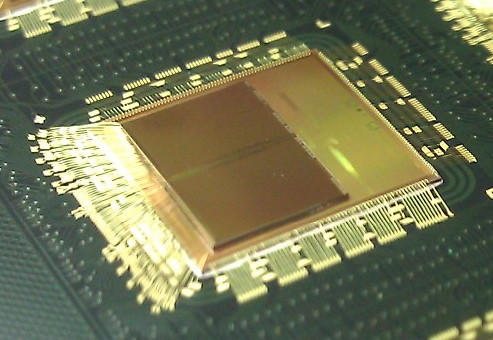
\includegraphics[width=0.25\linewidth]{images/spinnaker_die.jpg}
	\caption{SDRAM stich-bonded to the underlying SpiNNaker die.}
	\label{fig:spin5}
\end{figure}

The physical hierarchy of the system has each node containing two silicon dies --- the SpiNNaker chip itself, plus the Mobile DDR (Double Data Rate) SDRAM, which is physically mounted on top of the SpiNNaker die and stitch-bonded to it. The nodes are packaged and mounted in a 48-node hexagonal array on a PCB, the full system requiring 1,200 such boards. In operation, the engine consumes at most 90~kW of electrical power. \textbf{Figure~\ref{fig:spin5}} shows a photograph of the basic building block (a 48-chip SpiNNaker board) for the million-core machine.

\begin{figure}[htbp]
	\centering
	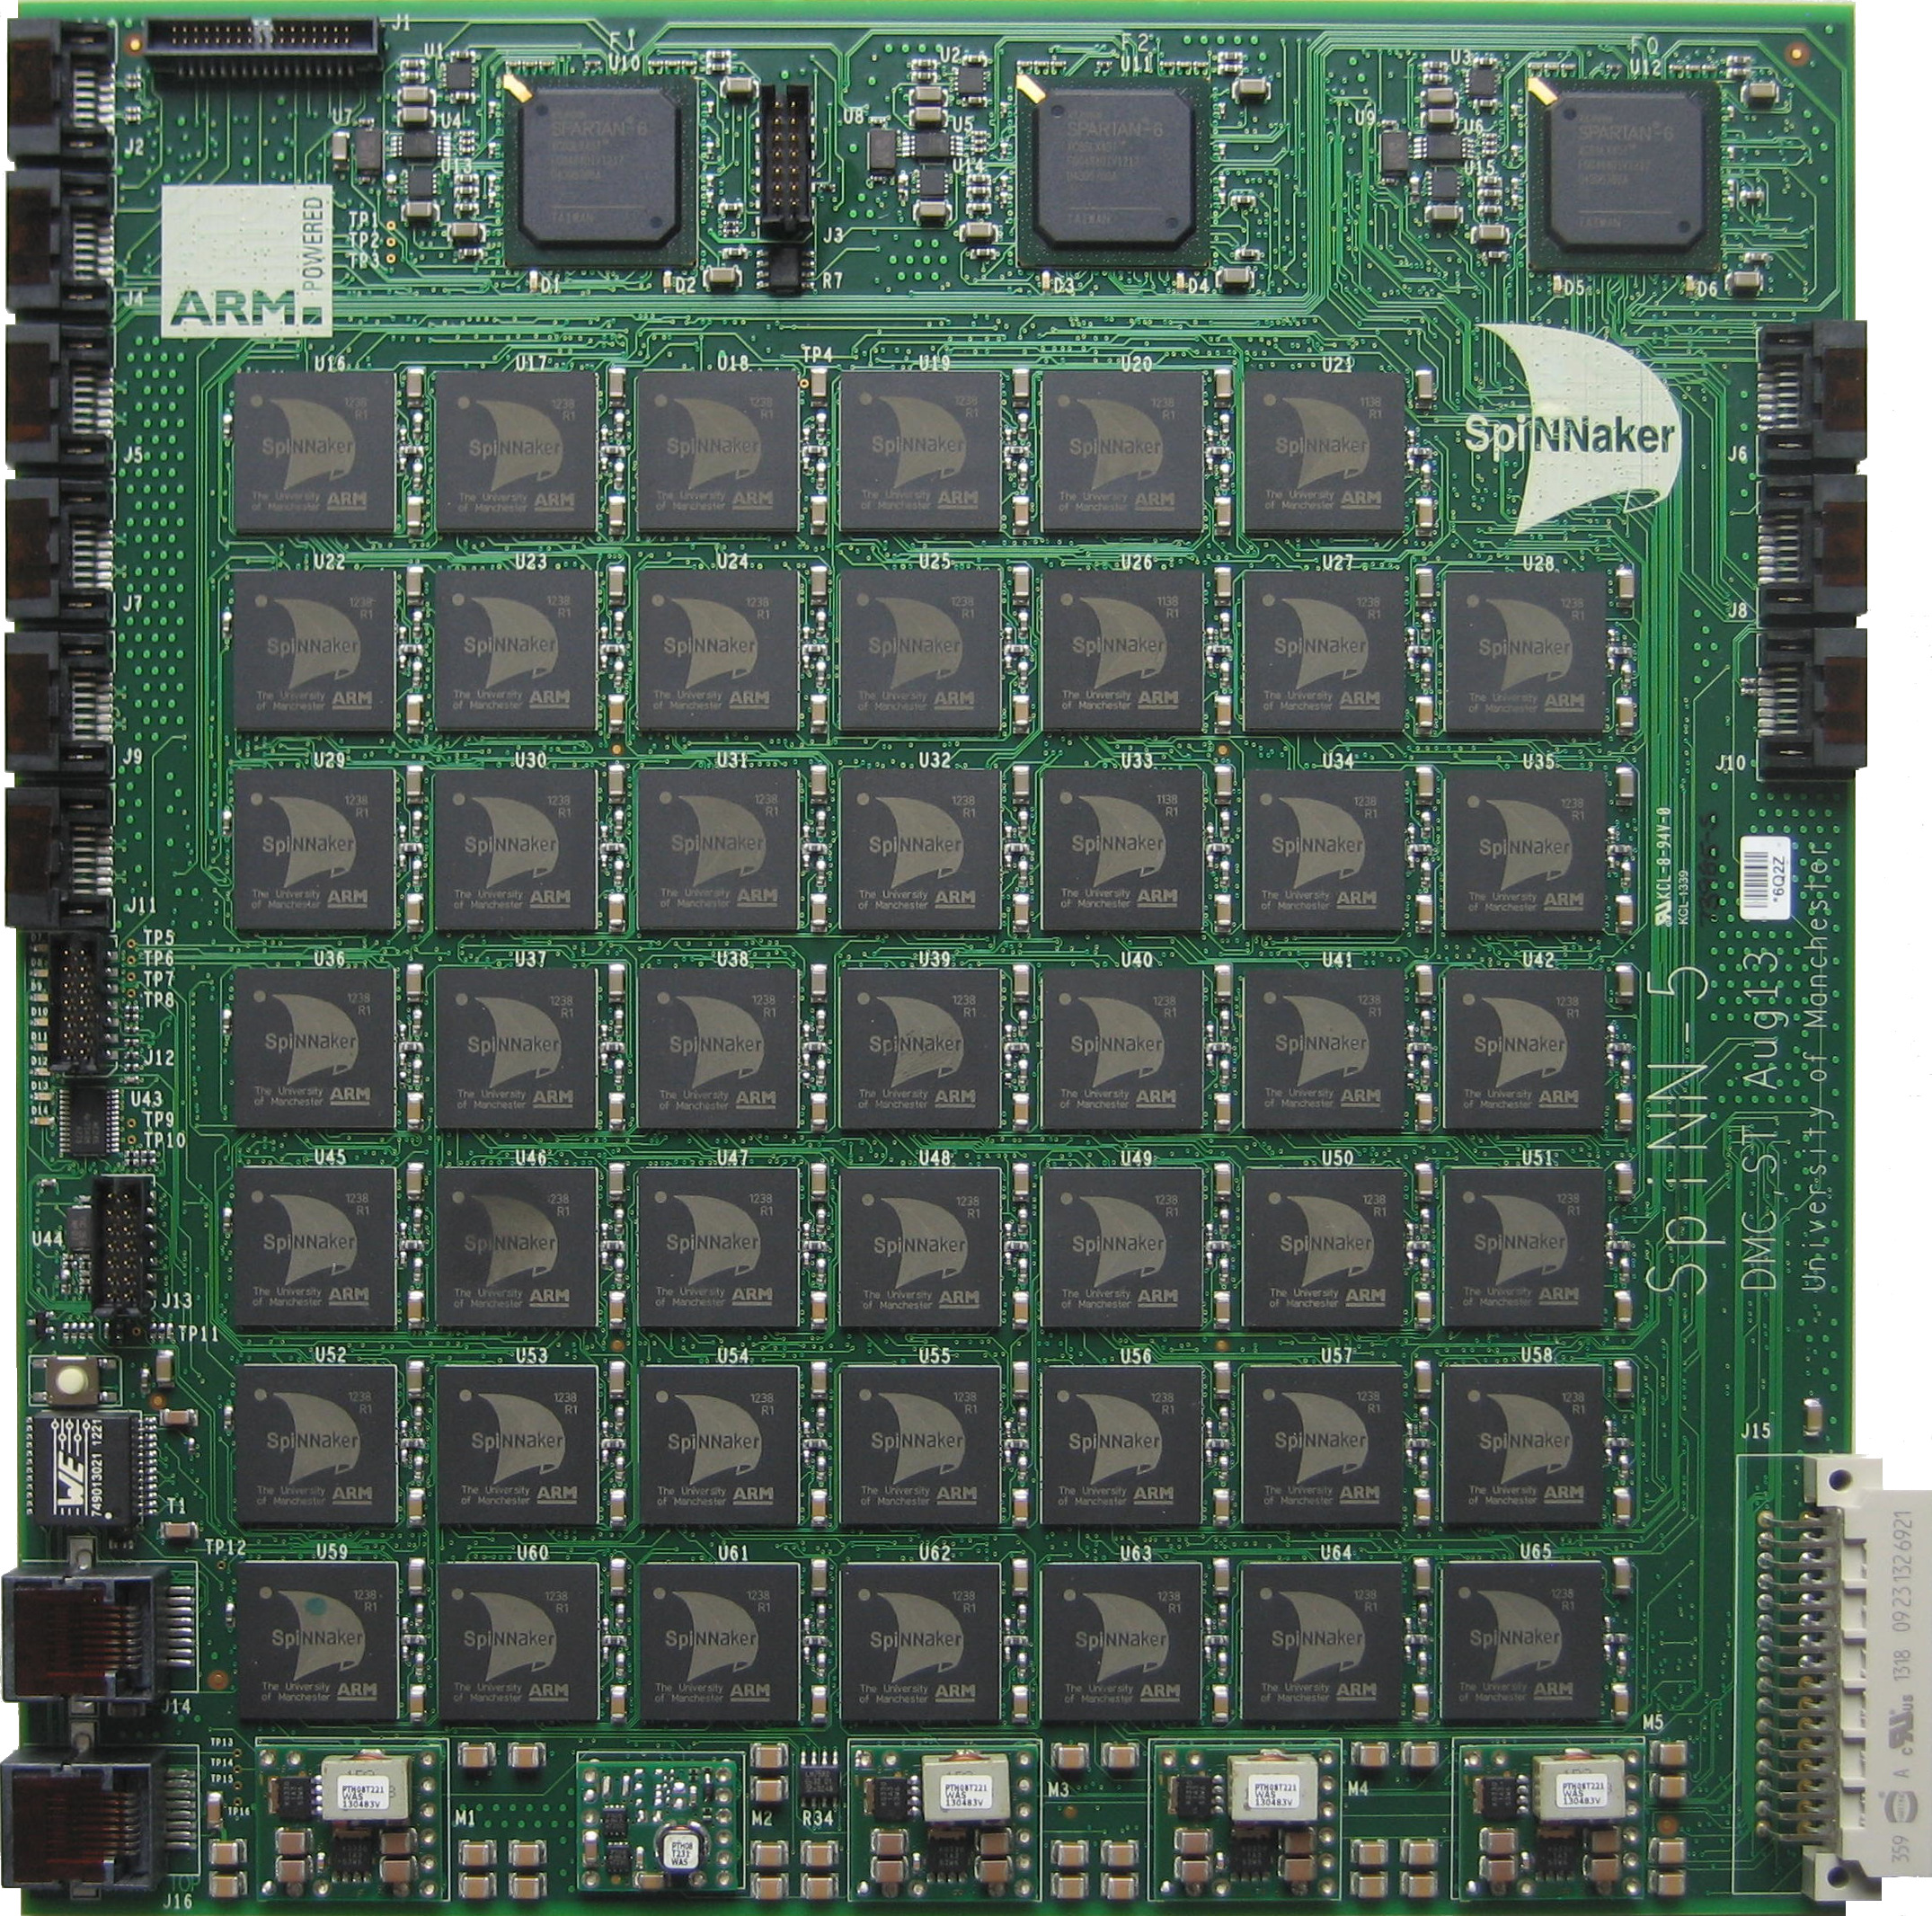
\includegraphics[width=0.45\linewidth]{images/spin5.jpg}
	\caption{48-chip Spin5 board}
	\label{fig:spin5}
\end{figure}

%\begin{figure}[htbp]
%	\centering
%	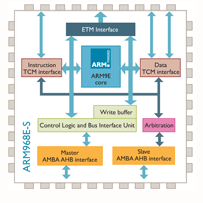
\includegraphics[width=0.2\linewidth]{images/arm968.png}
%	\caption{ARM968 architecture}
%	\label{fig:spin5}
%\end{figure}

\subsubsection{Hardware fault tolerance mechanisms in the SpiNNaker chip}
The SpiNNaker chip has been designed with fault tolerance in mind. The SpiNNaker chip is made up of various blocks, most of which have a certain degree of hardware fault tolerance in place. The blocks in questions are: the ARM968, the vector interrupt controller, the counter/timer, the DMA controller, the communications controller, the router, the inter-chip transmit and receiver interfaces, the SDRAM interface, the Ethernet interface, the system RAM and the boot ROM. A schematic representation of all these sub systems is shown in \textbf{Figure~\ref{fig:spin_arch}} and \textbf{Figure~\ref{fig:arm968}}.

\subsubsubsection{Block description}
\begin{itemize}
	\setlength\itemsep{-2pt}
	\item The \textbf{ARM968} together with the tightly-coupled instruction and date memories, forms the core processing resource in SpiNNaker.
	\item Each processor node on an SpiNNaker chip has a \textbf{vectored interrupt controller} (VIC) that is used to enable  and disable  interrupts  from  various  sources,  and  to wake  the processor  from  sleep mode when required. The interrupt controller provides centralised management of IRQ and FIQ sources, and offers an efficient indication of the active sources for IRQ vectoring purposes.
	\item Each processor node on a SpiNNaker chip has a \textbf{Counter/Timer}.
	\item Each ARM968 processing subsystem includes a \textbf{DMA controller}. The DMA controller is primarily used for transferring inter-neural connection data from the SDRAM in large blocks in response to an  input  event  arriving  at a  fascicle processor, and  for  returning updated connection data during learning. In addition, the DMA controller can transfer data to/from other targets on the System NoC such as the System RAM and Boot ROM. As a secondary function the DMA controller incorporates a `Bridge' across which its host ARM968 has direct read and write access to System NoC devices, including the SDRAM. The ARM968 can use the Bridge whether or not DMA transfers are active.
	\item	\textbf{Communications controller} --- Each processor node on SpiNNaker includes a communications controller which is responsible for generating and receiving packets to and from the communications network.
	\item The \textbf{Router} is responsible for routing all packets that arrive at its input to one or more of its outputs. It  is  responsible  for  routing multicast neural event packets, which  it does  through an associative multicast  router  subsystem,  point-to-point  packets  (for  which  it  uses  a  look-up  table),  nearest-neighbour packets  (using  a  simple  algorithmic process),  fixed-route packet  routing  (defined  in  a register), default routing (when a multicast packet does not match any entry in the multicast router) and emergency routing (when an output link is blocked due to congestion or hardware failure).\\
	Various error conditions are identified and handled by the Router, for example packet parity errors, time-out, and output link failure.
	\item \textbf{Inter-chip  communication}  is  implemented  by  extending  the Communications NoC  from  chip  to chip.  In  order  to  sustain  throughput,  there  is  a  protocol  conversion  at  each  chip  boundary  from standard CHAIN 3-of-6 return-to-zero to 2-of-7 non-return-to-zero. The interfaces include logic to minimise the risk of a protocol deadlock caused by glitches on the inter-chip wires.
	\item The \textbf{SDRAM  interface}  connects  the System NoC  to  an off-chip SDRAM device.  It  is  the ARM PL340, described in ARM document DDI 0331D.
	\item \textbf{Ethernet interface} --- The  SpiNNaker  system  connects  to  a  host  machine  via  Ethernet  links.  Each  SpiNNaker  chip includes  an  Ethernet MII  interface,  although  only  a  few  of  the  chips  are  expected  to  use  this interface. These chips will require an external PHY.\\
	The interface hardware operates at the frame level. All higher-level protocols will be implemented in software running on the local monitor processor.
	\item The \textbf{System RAM} is an additional 32 Kbyte block of on-chip RAM used primarily by the monitor processor to enhance its program and data memory resources as it will be running more complex (though less time-critical) algorithms than the fascicle processors.\\
	As the choice of monitor processor is made at start-up (and may change during run-time for fault-tolerance  purposes)  the  system  RAM  is  made  available  to  whichever  processor  is  monitor processor via  the System NoC. Accesses by  the Monitor Processor  to  the System RAM are non-blocking as far as SDRAM accesses by the fascicle processors are concerned.\\
	The System RAM may also be used by  the fascicle processors to communicate with  the monitor processor and with each other, should the need arise.
	\item The \textbf{Boot ROM} consists of a 32Kbyte on-chip ROM to provide minimal support for initial self-test and monitor processor selection. It also provides support for router initialisation for bootstrapping and system boot.
\end{itemize}

\begin{figure}[t]
	\centering
	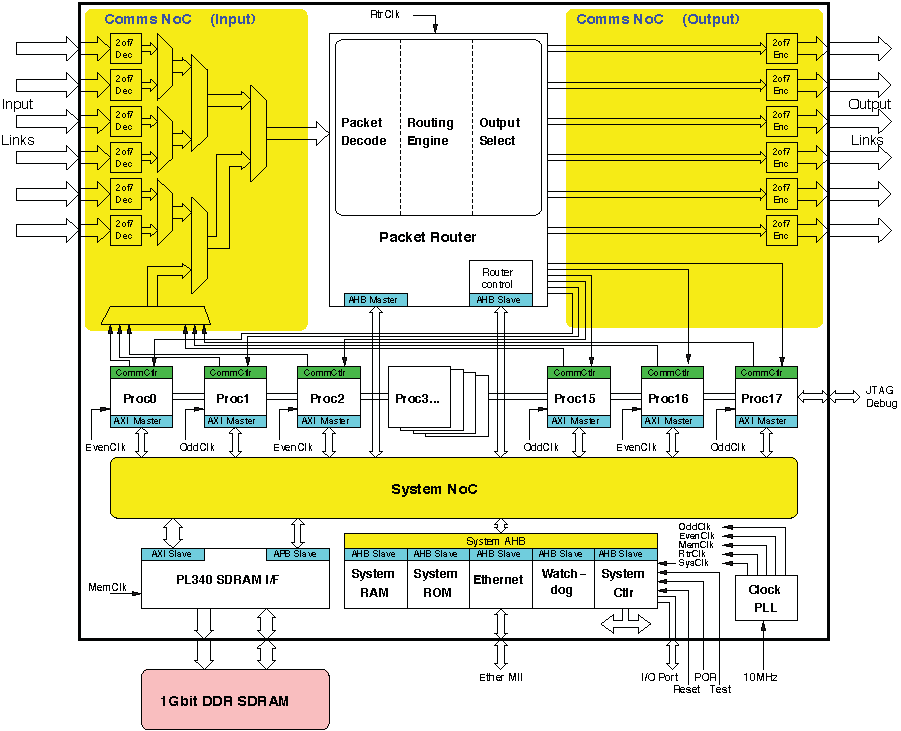
\includegraphics[width=0.7\linewidth]{images/spinnaker_architecture.pdf}
	\caption{SpiNNaker architecture}	
	\label{fig:spin_arch}
\end{figure}

\subsubsubsection{Fault tolerance mechanisms on SpiNNaker}
Starting by describing the fault tolerance detection mechanisms of the \textbf{ARM968} processor core, self-test routines are run at start-up and during normal operation. A chip-wide watchdog timer catches runaway software. In addition the ARM968 is able to isolate defective instruction and data RAM locations and can be mapped out by software. The system controller can also disable any incorrectly operating ARM968 cores. These detection and fault isolation mechanisms help to reconfigure the system in case a fault is detected. In the case of faulty instruction and data RAM, software can be written to avoid such locations. If on the other hand, the self-test and start-up routines detect a failure, the processor core functionality can be migrated to a neighbouring processor.

Currently the \textbf{vector interrupt controller} does not provide a high degree of fault tolerance. In the case of a failed vector location, the vector interrupt controller effectively jumps to a random location. If a software mechanism was devised to detect these kind of faults, a failed vector location could be removed from service (provided there are enough vector locations available). Another solution would be to shut down the entire vector system and the interrupts run by software inspection of the IRQ and FIQ status registers.

In order to detect faults in \textbf{counter/timer}, the second counter/timer could be configured with a longer period to check the calibration of the first. Assuming that the system only requires one counter/timer, and a fault is detected, the faulty counter could be disabled, with the operational counter/timer taking over.

\begin{figure}[t]
	\centering
	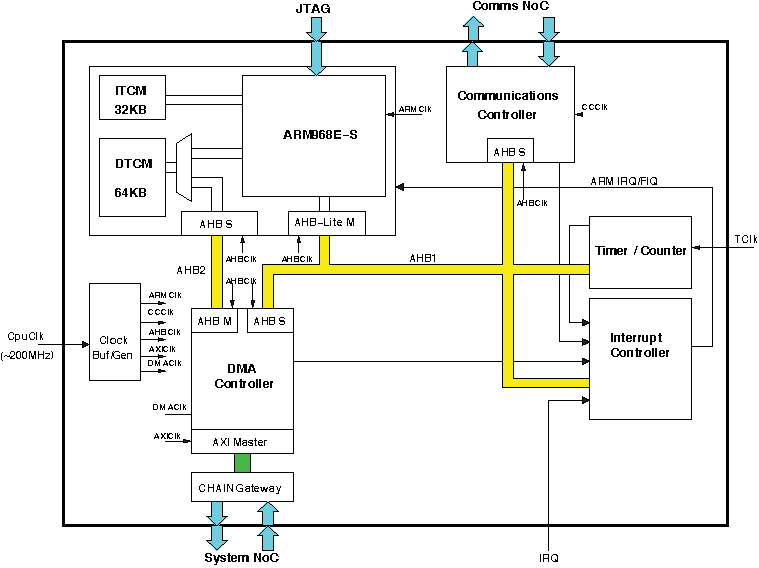
\includegraphics[width=0.7\linewidth]{images/arm968_subsystem.pdf}
	\caption{ARM 968 subsystem}
	\label{fig:arm968}
\end{figure}

The \textbf{DMA controller} has a CRC unit (more on this in \textbf{Section \ref{sec:crc}} which can be used to detect errors in the data transferred by the DMA controller. If an error is detected by means of the CRC unit, the data block could be retransmitted. The DMA controller will also time-out if a transaction takes too long. If if the error rate is consistently high, fault tolerant software could be written to shut down te local processing subsystem and its functions migrated to another subsystem on the current or to another chip.

The \textbf{communications controller} is able to detect the following kinds of faults:
parity of received packet; received packet framing error; transmit buffer overrun. Since the communications controller is mission-critical to the local processing subsystem, is should be disabled and isolated and its functions migrated to another subsystem on the current on onto another chip if a failure is detected.

\hl{The router section needs to be reorganized and put references to the backpressure and dropped packet reinjection sections}\\
The \textbf{router} is a sophisticated piece of circuitry and is endowed with some internal fault-tolerance capacity. In particular it is possible to map out a failed multicast router entry --- useful since the multicast router dominates the silicon area of the communications router. It also has the capacity to cope with external failures. Emergency routing will attempt to bypass a faulty or blocked link. In the event of a node (or larger) failure this will not be sufficient. In order to tolerate a chip failure several expedients can be employed on a local basis:
\begin{itmz}
	\item Point-to-point packets can be routed around the obstruction;
	\item Multicast packets with a router entry can be redirected appropriately.
\end{itmz}
In most cases, default multicast packets cannot sensibly be trapped by adding table entries due to their (almost) infinite variety. To allow re-routing, these packets can be dropped to the monitor processor on a link-by-link basis using the diversion register. In principle they can then be routed around the obstruction as point-to-point payloads before being resurrected at the opposite side. Should the monitor processor become overwhelmed, it is also possible to use the diversion register to eliminate these packets in the router; this prevents them blocking the router pipeline while waiting for a time-out and thus delaying viable traffic.

The router is able to detect the following faults --- packet parity errors, packet time-phase errors, packet unroutable errors such as a locally-sources multicast packet which doesn't match any entry in the multicast router, wrong packet length. In the case any of the above faults are detected, a multicast router entry can be disabled. The router can also be reconfigured to get around certain faults. For example, since all multicast router entries are identical the function of any entry can be relocated to a spare entry. Also, if a router becomes full a global reallocation of resources can move functionality to a different router.

\hl{Check the inter-chip Tx/Rx section}\\
The \textbf{inter-chip transmit and receive interfaces} (See \textbf{Figure~\ref{fig:interchip_links}}) has various fault detection capabilities, namely: Monitor processors should regularly test link functionality, an input controlled by the system controller causes the interface to deadlock, and the interface can be disabled to isolate the chip-chip link. As regards reconfiguration capabilities the link interface can be reset by the system controller to attempt recovery from the fault, and the link interface can be isolated and an alternative route used.

The fault inducing, detecting and resetting functions are controlled from the system controller. The interfaces are `glitch hardened' to greatly reduce the probability of a link deadlock arising as a result of a glitch on one of the inter-chip wires. Such a glitch may introduce packet errors, which will be detected and handled elsewhere, but it is very unlikely to cause deadlock. It is expected that the link reset function will not be required often.

The \textbf{SDRAM interface} is endowed with Delay-Locked Loop (DLL) delay lines (including a spare) which can be tested for stuck-at faults and relative timing accuracy. If a fault in the timing is detected, the SDRAM interface can be isolated and replaced by using the spare delay line.

The \textbf{Ethernet MII interface} is only used in a small number of nodes, specifically one for each group of 48 chips and thus most nodes are insensitive to faults in nuts functionality as they will not attempt to use it.

To detect faults in the \textbf{system RAM}, the monitor processor could perform a system RAM test at start-up, and also periodically during the course of the system operation. Since the system RAM does not employ any kind of parity or ECC system, it is not clear at this point to detect soft errors. If an error is detected through the start-up test, fault words could be mapped out of use. If the system RAM is deemed unusable, the only other option (short of completely disabling the entire chip) would be to use the SDRAM instead. This will probably result in compromised performance for the fascicle processors due to loss of SDRAM bandwidth.

A fault in the \textbf{boot ROM} can be easily detected during start-up if the boot ROM fails the boot process. One can easily switch the boot ROM out of the boot area rendering it harmless. When the boor ROM is switched out of the boot area the system RAM is switched in the boot area and a neighbour chip can initialise the system RAM with the boot code and retry initialisation.




%\begin{figure}[htbp]
%	\centering
%	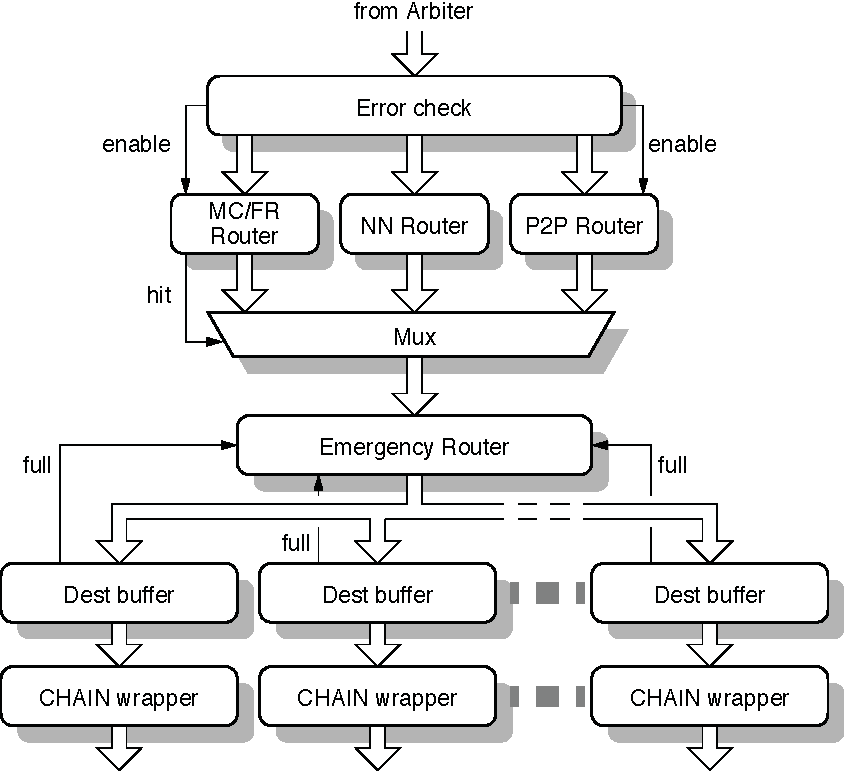
\includegraphics[width=0.6\linewidth]{images/router_organization.pdf}
%	\caption{Router organization}	
%\end{figure}

\clearpage
\section{Network congestion}

\subsection{Backpressure}
Backpressure visualisation. \textbf{Figure~\ref{fig:backpressure}} generated by 'Network Tester' \citep[see][]{heathcote2015networktester}.
\begin{figure}[htbp]
	\centering
	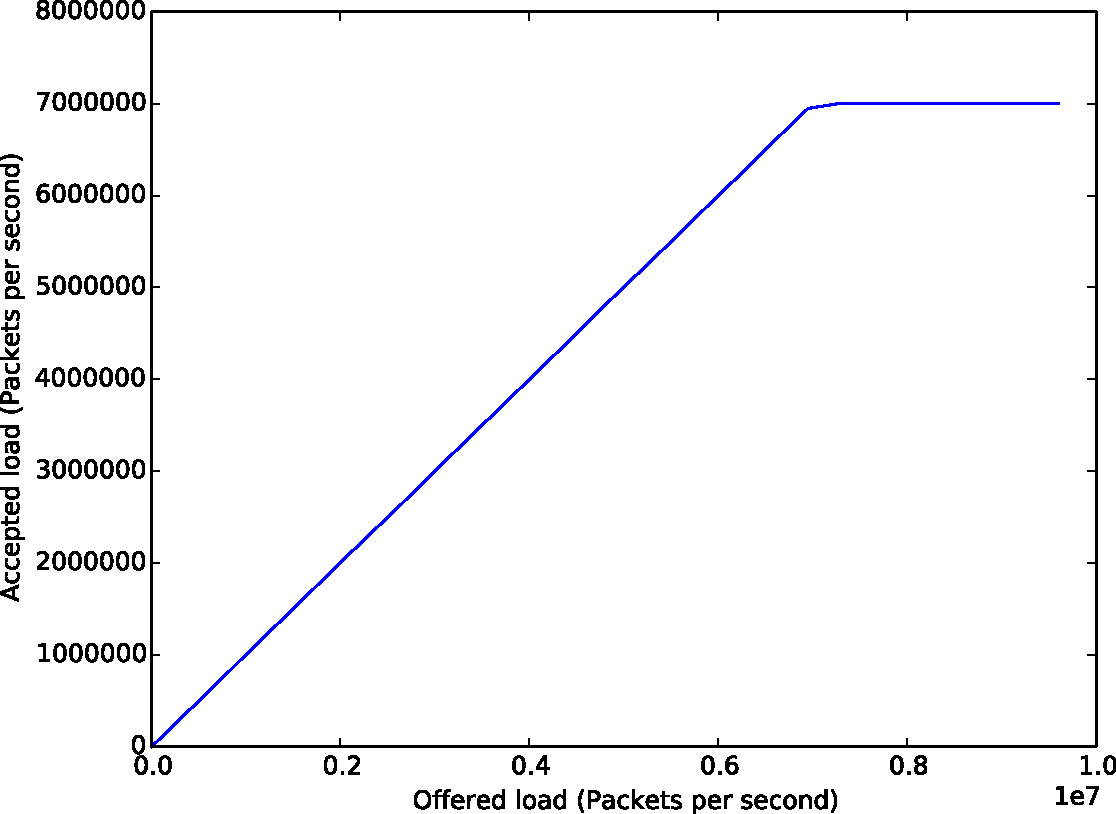
\includegraphics[width=0.5\linewidth]{images/backpressure2.pdf}
	\caption{Backpressure}	
	\label{fig:backpressure}
\end{figure}

\subsection{Dumped-packet reinsertion}
\begin{figure}[b]
	\centering
	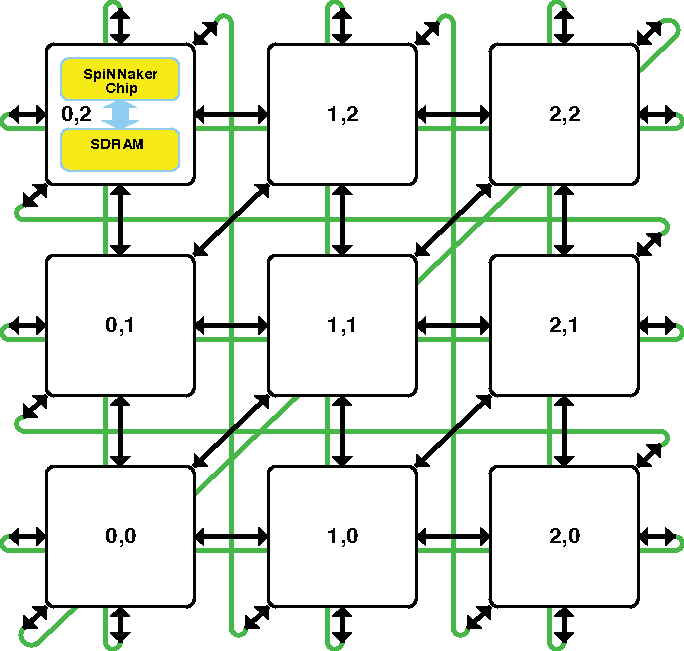
\includegraphics[width=0.35\linewidth]{images/system_architecture.pdf}
	\caption{SpiNNaker inter-links.}
	\label{fig:interchip_links}	
\end{figure}

`Network Tester' written by \citet{heathcote2015networktester} is a library designed to enable experimenters to quickly and easily describe and run experiments on SpiNNaker's interconnection network. In particular, network tester is designed to make recreating traffic loads similar to typical neural software straight-forward. Such network loads feature a fixed set of vertices (cores) which produce SpiNNaker packets which are then multicast to a fixed set of vertices.
The following is a (non-exhaustive) list of the kinds of experiments which can be performed with `Network Tester':
\begin{itemize}
\item Determining how a network copes with different rates and patterns of packet generation. For example to determining the maximum speed at which a particular neural simulation may run on SpiNNaker without dropping
packets.
\item Determining the effectiveness of place and route algorithms by finding `hot-spots' in the network.
\item Characterising the behaviour of the network in the presence of locally and globally synchronised bursting traffic.
\end{itemize}

\begin{figure}
	\begin{subfigure}[htbp]{.5\linewidth}
		\centering
		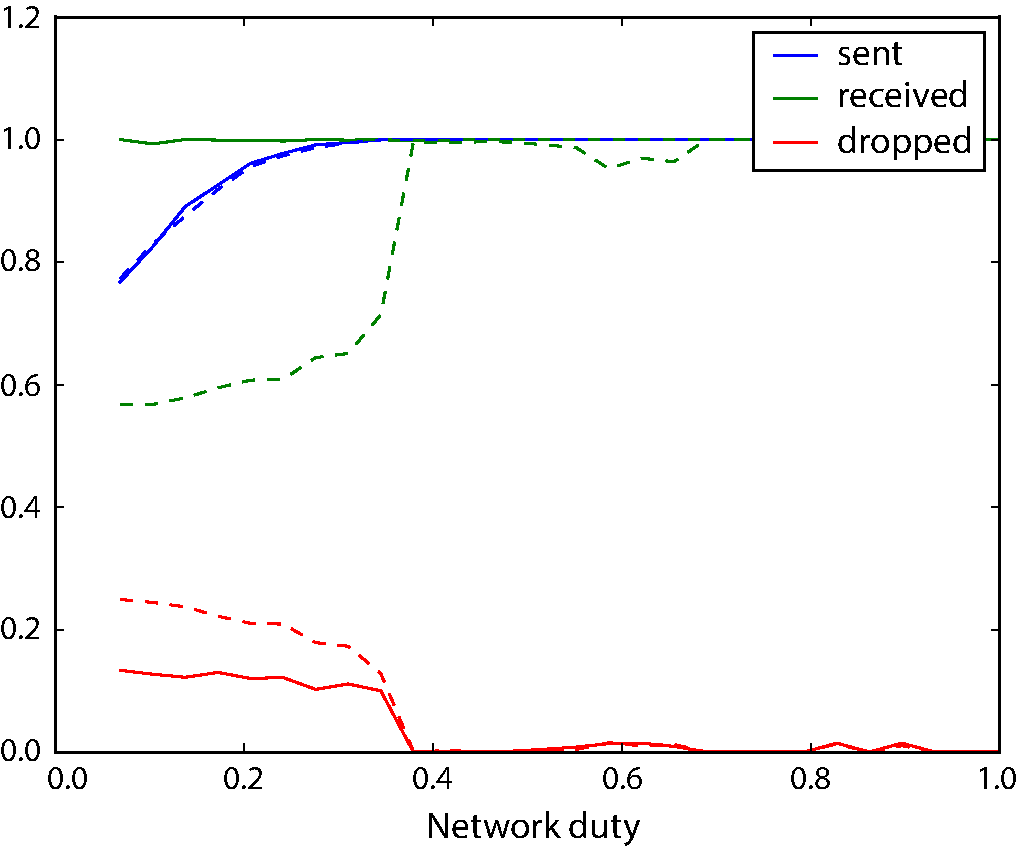
\includegraphics[width=0.9\linewidth]{images/bursting.pdf}
		\caption{Bursting}
		\label{fig:bursting}
	\end{subfigure}
	\begin{subfigure}[htbp]{.5\linewidth}
		\centering
		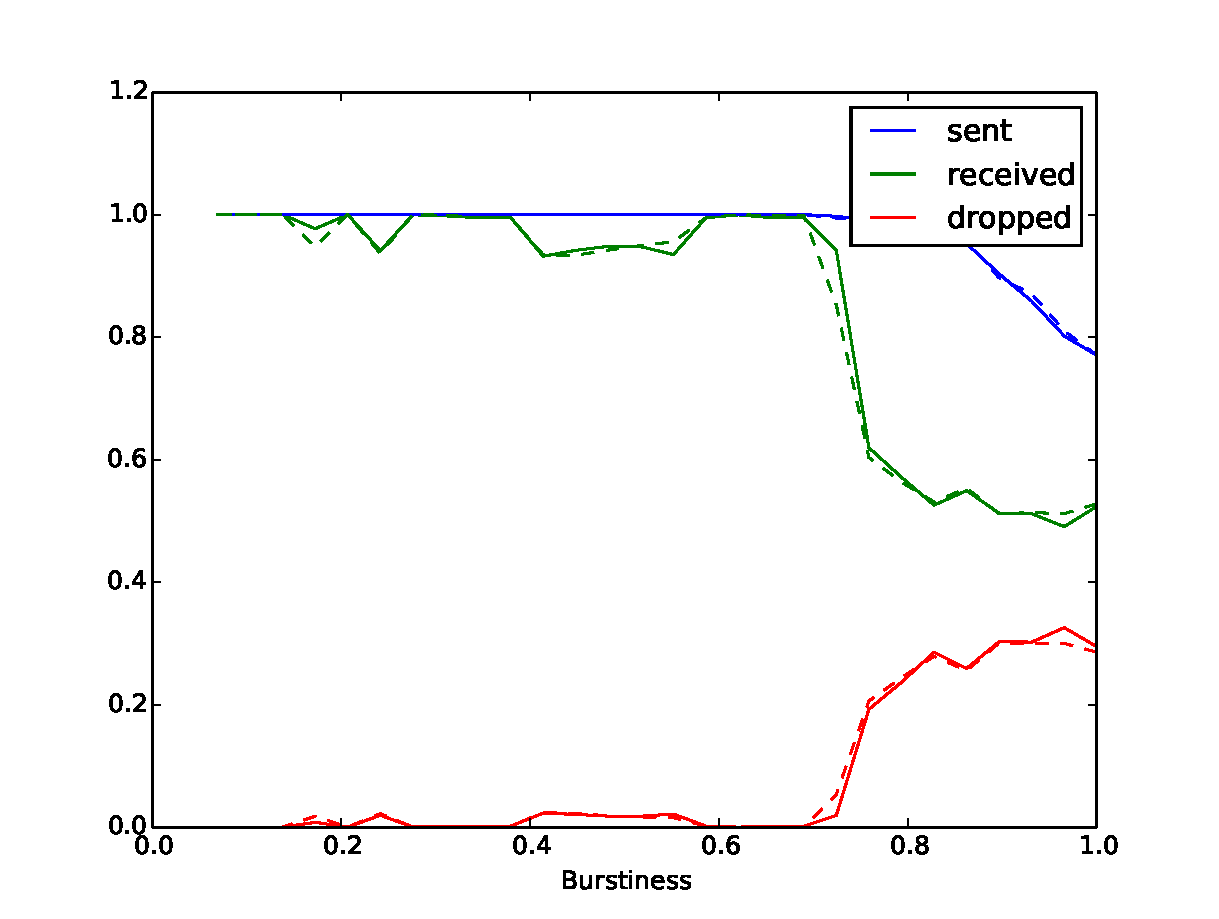
\includegraphics[width=0.9\linewidth]{images/bursting_connaware2.pdf}
		\caption{Bursting Connection-aware}	
		\label{fig:bursting_aware}
	\end{subfigure}
	\caption{Network congestion with respect to network load.}
\end{figure}


Clearly with packet reinjection, nearly all packets which are actually sent arrive at their destination, without reinjection, things aren't so great.

Fun things to try: Uncomment lines 23--24 and the random network will get placed by what PACMAN calls ``connectivity-aware placement,'' rather than simulated annealing (the default). Interestingly, on my system this results in reinjection no-longer helping and the whole thing being even worse under bursty packets.

Add the line \verb|e.burst_phase = None| somewhere before \verb|e.run()| is called and the packet generators will still generate bursts but they'll be at random phases to each other (i.e., not bursting all at the same time). This normally eliminates packet dropping for all but the most extreme burstiness.

\begin{figure}[htbp]
	\centering
	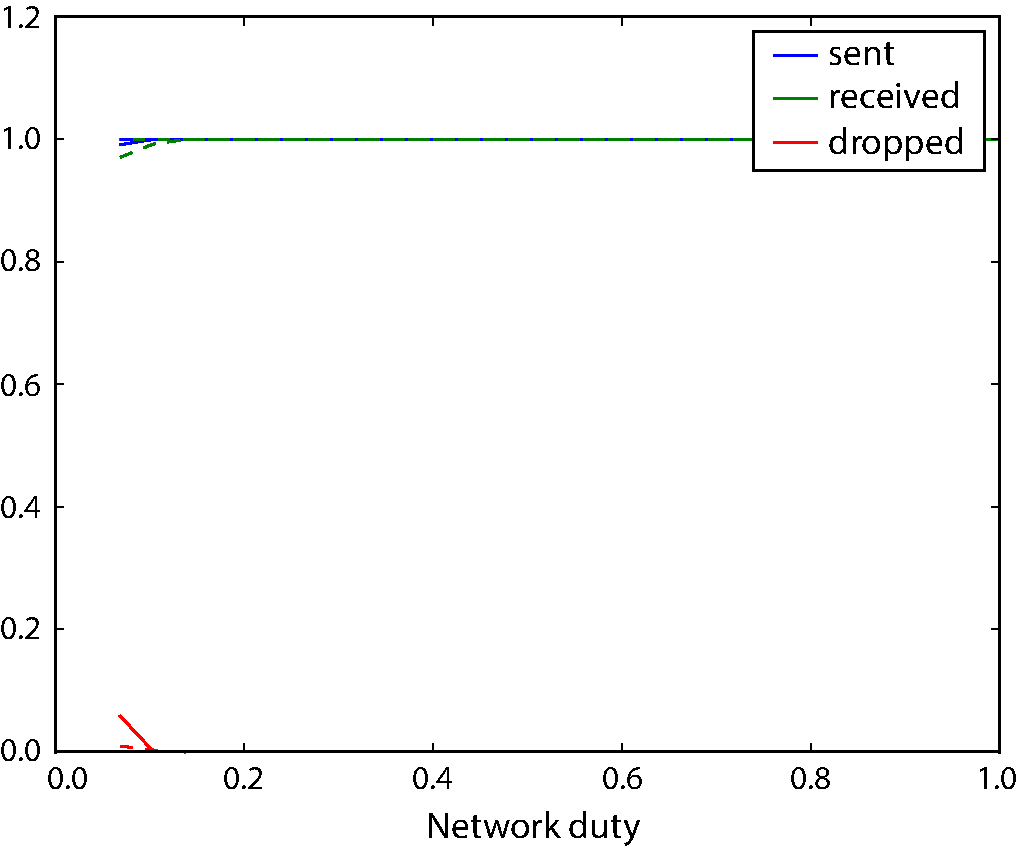
\includegraphics[width=0.5\linewidth]{images/bursting_random.pdf}
	\caption{Network congestion in a bursty (random) situation.}	
	\label{fig:bursting_random}
\end{figure}

\clearpage
\section{Process migration}
The heat demo is essentially a 2D heat diffusion equation solver (developed by Luis A. Plana). The heat equation is a partial differential equation that describes the variation in temperature over time in a region, given an initial temperature distribution and the boundary conditions. For a temperature $u(x,y,t)$ of two spatial variables $x$ and $y$ and the time variable $t$, the 2D heat equation is:
\[
\dpd{u}{t} -\alpha\left( \dpd[2]{u}{x} + \dpd[2]{u}{y} \right) = 0 
\]
where $\alpha$ is the thermal diffusivity, a material-dependent positive constant. A common way to solve this equation numerically is to approximate the derivatives by finite differences, generating a finite-difference discretisation of the heat equation.

Relaxation methods are iterative numerical methods used to solve systems of equations, including non-linear systems. In particular, they are commonly used to solve finite-difference discretisations of differential equations, such as the heat equation. A time-stepping algorithm is used to compute the new temperature of each point in the region, based on its current temperature and that of its neighbouring points:

\begin{align*}
\Delta x   &= \beta_x \cdot [u(x+1,y,t) + u(x-1,y,t) - 2 \cdot u(x,y,t)] \\
\Delta x   &= \beta_y \cdot [u(x,y+1,t) + u(x,y-1,t) - 2 \cdot u(x,y,t)] \\
u(x,y,t+1) &= u(x,y,t) + \Delta x + \Delta y
\end{align*}

\noindent A visualisation of the above equations is depicated in \textbf{Figure~{\ref{fig:heatdemo_iterative}}}.
\begin{figure}[htbp]
	\centering
	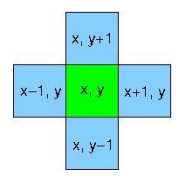
\includegraphics[width=0.2\linewidth]{images/heatdemo_iterative.png}
	\caption{2D heat diffusion --- finite difference method.}	
	\label{fig:heatdemo_iterative}
\end{figure}

These methods are well-suited for parallel implementation following a Single Program, Multiple Data (SPMD) model in which multiple autonomous cores simultaneously execute the same program with different data, and use messages to communicate with each other. In the heat equation case, each point sends its temperature to four neighbours and receives their temperatures in each time step.

Using a relaxation method to solve the heat equation is easily and efficiently mapped to SpiNNaker. In particular, the communications pattern is that which SpiNNaker is optimised for: many short messages sent concurrently to several destinations.

To implement the algorithm in SpiNNaker, the entire region is partitioned into sub-arrays of points and distributed across the machine. In the extreme case, every core is assigned a single point. Each core can then compute the corresponding temperatures and distribute them to its neighbours using SpiNNaker's efficient multicast communication infrastructure.

In SpiNNaker, the topology of the problem is dissociated from the topology of the machine, i.e., the mapping of points to cores in SpiNNaker is completely flexible and neighbouring points may not be mapped to neighbouring chips. Once the routing tables have been setup by the programme, a core can send a message with its current temperature and the communications infrastructure is responsible for the delivery of that message to the correct places.

SpiNNaker promotes event-driven software: cores respond to events and carry out the necessary computations. In the mean time, the cores are in low-power mode to save energy. Polling and idle iterations are avoided. In the heat equation solver, the arrival of a neighbour's temperature and the lapse of the time interval will trigger a core into operation.

\begin{figure}[htbp]
	\centering
	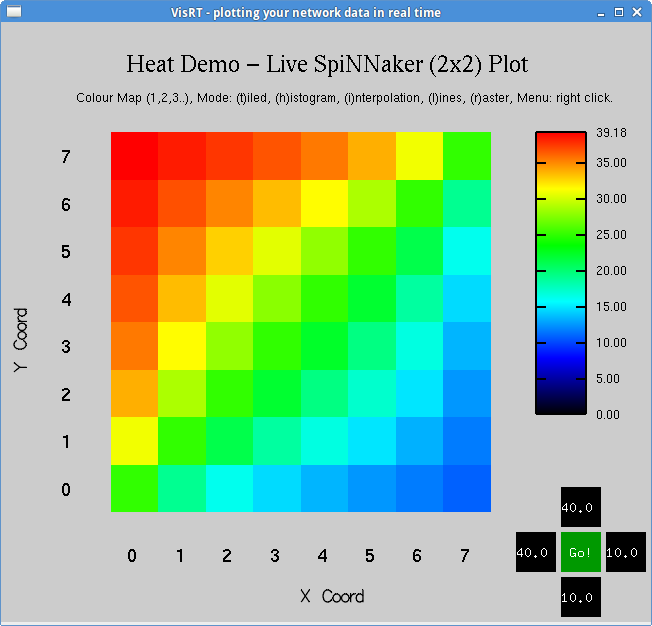
\includegraphics[width=0.6\linewidth]{images/heatmap2x2.png}
	\caption{Heat map demo visualisation on a 4-chip SpiNNaker board.}	
\end{figure}

The figure shows a snapshot of the output visualizer of a 2D Heat Diffusion Solver running on a 64-core SpiNNaker board. In this example, each of the 64 application cores in SpiNNaker is assigned a single point in a ``hexagonal'' region. Each square in the plot represents the temperature at a given point in the region.

The user can control the temperatures of the North, South, East and West boundaries and view the evolution of temperatures over time. The figure shows a scenario in which the North and West boundaries have been set to 40~\textdegree C and the East and South boundaries to 10~\textdegree C.

To test out the \verb|heat_demo_ft| functionality, start the \verb|heat_demo_ft.aplx|
by running (from ybug) \verb|@ heat_demo_ft_1board.ybug|

Then start resetting cores one-by-one by writing directly to the system
controller register \verb|(0xe2000000:r1 = 0xe2000004)|\\
Command: \verb|sw 0xe2000004 0x5ec00002|

Note: If the core you reset happens to be the leadAp, the application will
crash.

\emph{Currently implemented on the heat demo, where a core fault is simulated by intentionally reset a core. Currently if core 1 on core (0,0) is reset or disabled no communication is possible with the host PC.}


\clearpage
\section{CRC error correction}
\label{sec:crc}

\subsection{Discrete logarithms}
In mathematics, a discrete logarithm is an integer k solving the equation $b^k = g$, where $b$ and $g$ are elements of a finite group. Discrete logarithms are thus the finite-group-theoretic analogue of ordinary logarithms, which solve the same equation for real numbers $b$ and $g$, where $b$ is the base of the logarithm and $g$ is the value whose logarithm is being taken.

Computing discrete logarithms is believed to be difficult. No efficient general method for computing discrete logarithms on conventional computers is known, and several important algorithms in public-key cryptography base their security on the assumption that the discrete logarithm problem has no efficient solution.

\subsubsection{Example}
Discrete logarithms are perhaps simplest to understand in the group $(\mathbf{Z}_p)^\times$. This is the group of multiplication modulo the prime $p$. Its elements are congruence classes modulo $p$, and the group product of two elements may be obtained by ordinary integer multiplication of the elements followed by reduction modulo $p$.

The $k$th power of one of the numbers in this group may be computed by finding its $k$th power as an integer and then finding the remainder after division by $p$. When the numbers involved are large, it is more efficient to reduce modulo $p$ multiple times during the computation. Regardless of the specific algorithm used, this operation is called modular exponentiation. For example, consider $(\mathbf{Z}_{17})^\times$. To compute $3^4$ in this group, compute $3^4 = 81$, and then divide 81 by 17, obtaining a remainder of 13. Thus $3^4 = 13$ in the group $(\mathbf{Z}_{17})^\times$.

The discrete logarithm is just the inverse operation. For example, consider the equation $3^k \equiv 13$ (mod 17) for $k$. From the example above, one solution is $k = 4$, but it is not the only solution. Since $3^{16} \equiv 1$ (mod 17)---as follows from Fermat's little theorem---it also follows that if $n$ is an integer then $3^{4+16n} \equiv 3^4 \times (3^{16})^n \equiv 13 \times 1^n \equiv 13 $ (mod 17). Hence the equation has infinitely many solutions of the form $4 + 16n$. Moreover, since 16 is the smallest positive integer $m$ satisfying $3m \equiv 1$ (mod 17), i.e. 16 is the order of 3 in $(\mathbf{Z}_{17})^\times$, these are the only solutions. Equivalently, the set of all possible solutions can be expressed by the constraint that $k \equiv 4 $  (mod 16).

\subsubsection{Algorithms}
No efficient classical algorithm for computing general discrete logarithms $\log _b g$ is known. The naive algorithm is to raise $b$ to higher and higher powers $k$ until the desired $g$ is found; this is sometimes called trial multiplication. This algorithm requires running time linear in the size of the group $G$ and thus exponential in the number of digits in the size of the group. There exists an efficient quantum algorithm due to Peter Shor.[1]

More sophisticated algorithms exist, usually inspired by similar algorithms for integer factorization. These algorithms run faster than the naive algorithm, some of them linear in the square root of the size of the group, and thus exponential in half the number of digits in the size of the group. However none of them runs in polynomial time (in the number of digits in the size of the group).

%\begin{itemize}
%\setlength{\itemsep}{0pt}
%\item Baby-step giant-step
%\item Function field sieve
%\item Index calculus algorithm
%\item Number field sieve
%\item Pohlig–Hellman algorithm
%\item Pollard's rho algorithm for logarithms
%\item Pollard's kangaroo algorithm (aka Pollard's lambda algorithm)
%\end{itemize}

\subsubsection{Comparison to integer factorization}
While computing discrete logarithms and factoring integers are distinct problems, they share some properties:

\begin{itemize}
	\setlength{\itemsep}{-2pt}
	\item both problems are difficult (no efficient algorithms are known for non-quantum computers),
	\item for both problems efficient algorithms on quantum computers are known,
	\item algorithms from one problem are often adapted to the other, and
	\item the difficulty of both problems has been used to construct various cryptographic systems.
\end{itemize}

\subsection{Abstract} --- Martin Grymel
Error-control codes provide a mechanism to increase the reliability of digital data being processed, transmitted, or stored under noisy conditions. Cyclic codes constitute an important class of error-control code, offering powerful error detection and correction capabilities. They can easily be generated and verified in hardware, which makes them particularly well suited to the practical use as error detecting codes.

A cyclic code is based on a generator polynomial which determines its properties including the specific error detection strength. The optimal choice of polynomial depends on many factors that may be influenced by the underlying application. It is therefore advantageous to employ programmable cyclic code hardware that allows a flexible choice of polynomial to be applied to different requirements. A novel method is presented in this thesis to realise programmable cyclic code circuits that are fast, energy-efficient and minimise implementation resources.

It can be shown that the correction of a single-bit error on the basis of a cyclic code is equivalent to the solution of an instance of the discrete logarithm problem. A new approach is proposed for computing discrete logarithms; this leads to a generic deterministic algorithm for analysed group orders that equal Mersenne numbers with an exponent of a power of two. The algorithm exhibits a worst-case runtime in the order of the square root of the group order and constant space requirements.

This thesis establishes new relationships for finite fields that are represented as the polynomial ring over the binary field modulo a primitive polynomial. With a subset of these properties, a novel approach is developed for the solution of the discrete logarithm in the multiplicative groups of these fields. This leads to a deterministic algorithm for small group orders that has linear space and linearithmic time requirements in the degree of defining polynomial, enabling an efficient correction of single-bit errors based on the corresponding cyclic codes.

\subsection{Introduction}
\ul{The preservation of digital data integrity is of major concern for computer, communication, and storage systems. In all these applications digital data is susceptible to unintentional modification which may arise from electrical or magnetic disturbance, component failure, or the result of system design error. Depending on the specific application, data failures may result in severe consequences and thus their potential occurrence needs to be considered carefully in the underlying design of the system.}

Data reliability can be enhanced through the employment of error-control codes,which provide mechanisms for the detection and correction of errors. These codes enrich the data with redundancy by forming code words, which initially can be used to detect inconsistencies in the received data. If the affected data can be retransmitted or recalculated, one simple error correction scheme is the Automatic Repeat Query (ARQ), where the receiver simply requests a retransmission once it detects data inconsistencies. However, where retransmission or recalculation is not feasible, being too slow or uneconomic, Forward Error Correction (FEC) techniques can correct errors on the basis of the corrupted received data and its inherent redundancy.

Cyclic codes form an important class of error-control code offering powerful error detection and correction capabilities. At the same time, their algebraic properties permit the use of simplified processing procedures when compared to non-cyclic codes. For instance, the encoding of data into cyclic code words can easily be achieved in hardware using a simple linear feedback shift register. Likewise, the same circuit can be used to validate code words, and thus detect errors. For these reasons, cyclic codes have been widely adopted as error-detecting codes and commonly deployed in combination with ARQ schemes. This thesis concentrates on cyclic codes with symbols from the binary field.

If error correction is desired, the most basic case concerns the localisation of a single erroneous bit. It can be shown that for cyclic codes this problem is equivalent to the computation of the discrete logarithm in finite cyclic groups, for which it is widely believed that for the general case no efficient classical algorithm is devisable. This is one reason why the discrete logarithm forms the basis for many cryptographic applications such as the Diffie-Hellman-Merkle key exchange. However, it has not been proven that the computation of the discrete logarithm is hard for all groups of practical interest.

Cyclic codes are characterised by an underlying generator polynomial. Different generator polynomials exhibit different capabilities in regard to the detection and correction of errors. Certain polynomials, for example,may be particularly well suited to the practical realisation of the error correction process. The selection of polynomial is also dependent on the length of the data that is to be protected and the anticipated error patterns. In systems where diverse applications may favour different cyclic codes, and where the requirements may change over time or be unknown at the design stage, it may be advantageous to provide full flexibility in regard to the usable cyclic code generator polynomials. Efficient cyclic code processing relies on dedicated cyclic code hardware circuits, which may be programmable if the underlying generator polynomial is adaptable. Such a programmable circuit has been created for the SpiNNaker project, a massively parallel spiking neural network simulator.

\subsection{Objectives}
Cyclic codes comprise a powerful class of error-control code; they have gained wide popularity in the field of error detection owing to their efficient hardware implementations and simultaneous effective error detection. Programmable cyclic code circuits have the benefit of flexible adaptation of the underlying cyclic code to meet the requirements of a specific application. One goal of this research is to provide a method for the efficient realisation of parallel programmable cyclic code circuits, in hardware, to make them appealing for a wider range of applications.

The current predominating drawback of cyclic codes is the lack of efficient error correction techniques for them. To perform the correction of a single-bit error an instance of the generalised discrete logarithm problem needs to be solved. It is an additional goal of this research to explore new methods in the quest for an efficient mechanism for computing discrete logarithms in relevant finite cyclic groups and, therefore, facilitate the efficient recovery from single-bit errors through cyclic codes.

\subsection{Contribution}
The contributions of this thesis are summarised as follows:

\begin{itemize}
\item A new scheme is proposed enabling the efficient calculation of the state transition and control matrix for the parallel operation of a cyclic code circuit in hardware. This circuit is used both for the data encoding step and the decoder error detection phase. With the incorporation of a programmable transition and control matrix, this adaptable circuit can be configured to use different cyclic codes. This added flexibility is a valuable enhancement, as the error detection and error correction performance of a particular cyclic code depends on parameters including the length of the data that is to be protected and the anticipated error patterns of an application. A simulation of the novel programmable cyclic code circuit produced shows significant improvements in terms of speed, area and energy efficiency when compared with previously published designs. The design of the new circuit has been published [GF11].
\item A new approach is proposed for the computation of discrete logarithms; this leads to a generic deterministic algorithm for analysed group orders that equal a Mersenne number where the exponent is a power of two. It is shown that, for these groups, the worst-case running time is proportional to the square root of the group order, while the space requirements are constant. The scheme is further improved for particular cases where the discrete logarithm values occur with different probabilities, leading to reduced average and worst-case execution times. Furthermore, properties are derived that apply to the sequences that are used by the algorithm.
\item A set of new relationships is developed for the field elements of the ring of polynomials over the binary field modulo a primitive polynomial. Based on a subset of these properties, a novel approach is proposed for the computation of discrete logarithms in the cyclic multiplicative group of the finite field. For at least all primitive polynomials up to degree 12 and the first evaluated primitive polynomials of degree 13 and 14, a deterministic algorithm with linear space and linearithmic time requirements in the degree of the polynomial results.
\end{itemize}

\subsection{Overview}
\subsubsection{Chapter 4}
This chapter presents an overview of the SpiNNaker project which targets the large-scale simulation of spiking neural networks. The SpiNNaker architecture facilitates a massively-parallel supercomputer with a million processors, which supports these neural simulations. The issue of anticipated memory faults in a SpiNNaker system of this scale is highlighted, and the usage of cyclic codes as a layer of protection against many of these errors is explained.

\subsubsection{Chapter 5}
In this chapter, the equations for a parallel realisation of a cyclic code circuit are derived. It is then shown how a programmable version of such a circuit can be created which can be configured to use different generator polynomials. Furthermore, a new scheme is presented that allows the efficient computation of the state transition and control matrix necessary for the circuit. With this scheme a novel programmable parallel cyclic code circuit is proposed that is then compared to previous work. This chapter is based on a journal publication [GF11].

\subsubsection{Chapter 6}
This chapter describes a new generic approach for the computation of the discrete logarithm. Based on this approach an algorithm is presented for group sizes that equal a Mersenne number with an exponent of a power of two. It is shown how the scheme can be improved if the discrete logarithm values occur with unequal probabilities. Properties are derived for the sequences that are used by the algorithm and finally, the proposed scheme is compared with an established method for the evaluation of discrete logarithms.

\subsubsection{Chapter 7}
In this chapter, a new set of properties is derived for the elements of a finite field with binary characteristic, where the field is represented as a polynomial ring over the binary field modulo a primitive polynomial. For the multiplicative group of the finite field, a novel approach is presented to compute discrete logarithms based on a subset of the newly established field properties. Performance results are reported for the resulting algorithm for evaluated small group sizes.


\subsection{Excerpts from Chapter 4 -- SpiNNaker}
\subsubsection{Memory}
The large SpiNNaker system in its envisaged configuration of 57,600 nodes will incorporate in the order of 7 TiB of SDRAM. With such an immense amount of memory, the effect of data bit errors is significant during the operation of the machine.

Memory bit errors are subdivided into two different classes: hard and soft errors [ZL79; Zie96; Zie+96].A hard error is characterised by a permanent hardware fault in a memory cell that will result in a consistent reliability issue. For instance, it may be the case that a memory cell will always provide one particular bit value during readout, no matter what value has been written to it. Soft errors are transient faults that occur randomly and may, for example, be induced through cosmic rays or the decay of radioactive atoms in the memory packaging materials. Also, a soft error may arise either directly in the memory, or along the data path during the memory read or write phase.

Recently, a large-scale study has been conducted to investigate statistics for error rates in Dynamic Random Access Memory (DRAM) in production systems [SPW09]. It suggests that the average error rate ranges from 25,000 to 75,000 FIT (failures in time per billion hours of operation) per Mibit, however a distinction between hard and soft errors is not made. If these numbers are applied to the SpiNNaker system of 57,600 nodes, 25 to 74 bit errors on average can be expected to occur within the SDRAM per minute, roughly approximated as one bit error per second.

It may be the case that the number of expected bit errors in the SpiNNaker system will not have a significant impact on particular applications such as neural network simulations. However, it is not known to what extent neural network simulations can compensate for memory faults, and other potential applications may not tolerate bit errors at all, so appropriate measures need to be taken to deal with them in the SpiNNaker system. For this reason error-control codes are employed within SpiNNaker to provide a layer of protection against memory faults.

\subsubsection{CRC unit}
The DMA controller of each processing subsystem has been equipped with a CRC unit that allows the generation and verification of error-control codes. The circuit primarily supports cyclic codes as they offer powerful error detection and correction capabilities and as they are, at the same time, easily implementable in hardware [LC83]. If, for instance, a processor initiates a DMA transfer to copy a data block from the local memory to the SDRAM, the CRC unit can be instructed to calculate (transparently and in parallel) the redundancy part for a cyclic code and, automatically, append this to the SDRAM data block. The CRC unit can be used to calculate the error syndrome for a data block retrieved from memory and signal the corresponding processing core if an integrity issue arose. The program that is executed on the processing core has to decide what action is to be taken in the event of a detected data inconsistency. A simple retransmission of the data block could correct the error if it occurred along the data path during the readout phase, however even this may not be fast enough for the `real-time' operation of a SpiNNaker neural simulation. Therefore it is necessary to consider appropriate error correction procedures in software, to recover from memory faults based on the obtained error syndrome, including when they are uncorrectable. These can range from a simple disregard of the error, through a localisation and correction of the error, to a shutdown of the relevant SpiNNaker system components for replacement if hard errors are involved.

In the choice of employed cyclic code, many factors need to be taken into account for the selection of the generator polynomial as outlined in Subsection 2.3.4. For instance, certain undiscovered subclasses of cyclic codes may allow the realisation of very efficient error correction procedures in software, or data blocks of different lengths may be stored in the SDRAM so that a polynomial offering best combined error protection for all of the block lengths should be selected. To offer maximal flexibility within SpiNNaker, a programmable CRC circuit has been incorporated that permits switching the generator polynomial to any of degree 32 or lower whenever required. A direct advantage is that the polynomial is adaptable to the length of the data block that is to be protected, which means that the best choice of offered error protection can be made. Another feature of the CRC circuit is that several cyclic codes of a smaller degree can be generated based on different bits of the data stream. For example, for each half-word of the data stream, a cyclic code based on a generator polynomial of degree 16 can be computed.

The width of the data bus that traverses the DMA controller in SpiNNaker is 32 bits, and the CRC unit has been designed to process this number of bits in parallel to avoid being a bottleneck to DMA data transfers. To configure the unit for the usage of a cyclic code or any other supported error-control code, one Kibit of configuration data needs to be supplied by the corresponding processing core to the appropriate registers inside the unit. Since the data bus is used to provide this configuration data, the transfer takes place as a series of 32 bit words. The registers are realised as latches to reduce the hardware demand, as each SpiNNaker chip accommodates one CRC unit for each of the 18 DMA controllers (one per processor subsystem). A detailed description of the SpiNNaker CRC circuit together with its derivation and capabilities can be found in the next chapter.

\subsubsection{Conclusion}
The SpiNNaker architecture has been created to support large-scale simulations of spiking neural networks in biological real-time. It has been dimensioned to scale up to machines consisting of a million processors with SDRAM totalling about 7 TiB. With such a vast amount of memory, it is estimated that, on average, about 1 bit error per second will occur.

To improve the reliability of memory transfers, SpiNNaker employs cyclic codes for error control due to the efficient realisation of the code generation and verification circuit. Once inconsistencies are detected for a block of data, software procedures may be triggered to attempt an error recovery. The correction of a single-bit error on the basis of a cyclic code, essentially requires the computation of the discrete logarithm in relevant groups as described in Chapter 2. However, no efficient algorithm is known for the computation of this type of discrete logarithm as discussed in Chapter 3. Two new solutions for the computation of the discrete logarithm in certain groups are proposed in Chapter 6 and Chapter 7.

The optimal choice of cyclic code to employ is influenced by many factors including the length of the data that is to be protected and the desired error control capabilities. Therefore, programmable cyclic code circuits are employed within SpiNNaker to maximise flexibility in the choice of cyclic code for different scenarios. A novel method for the generation of efficient programmable cyclic code circuits is proposed in Chapter 5.

\newpage
\subsection{Excerpts from Chapter 5 --- Programmable CRC hardware}
Cyclic codes constitute a powerful class of error-control code as set out in Section 2.3. They offer effective error detection and can easily be realised in hardware, which makes them a popular choice for many applications that require the detection of errors, including Ethernet [TW11]. In the context of pure error detection, a cyclic code is often referred to as a Cyclic Redundancy Checksum (CRC) and the popularity of cyclic codes has led to a number of different software and hardware implementations [LC83; RG88].Speed requirements usually make software schemes impractical and dedicated hardware is needed. The generic hardware approach uses an inexpensive Linear Feedback Shift Register (LFSR), which assumes serial data input. In the presence of wide data buses, the serial computation has been extended to parallel versions that process whole data words based on derived equations and on cascading the LFSR [Spr01]. Various optimisation techniques have been developed that target resource reduction [Bra+96] and speed increase [Der01; CP06; KRM08; KRM09].

A wide range of factors influence the selection of an appropriate CRC generator polynomial for a particular application as outlined in Subsection 2.3.4. This range includes the error detection and correction capabilities of a generator polynomial, which depend on the length of the data that is to be protected. For instance, in scenarios where data blocks of different length are used, or where the final requirements of the generator polynomial are not known at the time of the hardware implementation, it is beneficial to employ programmable CRC circuits that can be configured to different generator polynomials.

This applies precisely to the SpiNNaker project, whose target is to provide a research platform for the simulation of arbitrary spiking neural networks as described in Chapter 4. The planned large SpiNNaker system will incorporate a substantial amount of SDRAM to hold relevant data for the neural network simulations; in this context, CRCs are used to reduce the effect of data errors arising in the memory. Since the length of the data blocks may vary between different neural network simulations, for instance, it has been decided to incorporate programmable CRC circuits into the SpiNNaker system to offer maximal flexibility.

With the design of a circuit, there is usually a tradeoff between speed and area. In this particular scenario, there are two dimensions to the speed of a programmable CRC circuit: the time necessary to process a data word, and the time required to reconfigure to a new polynomial. This chapter directly extends the parallel CRC circuit by Campobello et al. [CPR03] based on state space representation in several ways. On the one hand, restrictions between the width of the data processed in parallel and the order of the polynomial are lifted. On the other hand, a novel scheme is presented allowing the inexpensive computation of the CRC transition and control matrix in hardware. This leads to a programmable parallel CRC implementation that offers an improved balance between area and both dimensions of speed.

\subsection{Excerpts from Chapter 8 Conclusion -- Cyclic codes}
Cyclic codes have gained wide popularity as error-detecting codes due to their inherent algebraic properties that permit easy implementation and effective detection of errors. This thesis supports the position of cyclic codes as a powerful class of error-control code whose properties extend beyond simple error detection. The thesis demonstrates contributions in the generation of efficient, programmable, parallel cyclic code circuits, and in the potential of cyclic codes for efficient error correction. These contributions are described in more detail, together with highlighting possible areas for future exploration within this concluding chapter.

\subsubsection{Programmable CRC}
A cyclic code is characterised through its generator polynomial which influences the specific error detection and correction capabilities of the code, depending on the length of the data that is to be protected, as outlined in Chapter 2. In addition, different applications may run on the same system with completely different cyclic code requirements, as in the case of SpiNNaker which is described in Chapter 4. It was shown how cyclic code circuits can overcome the limitations of a single generator polynomial by allowing the circuit to be flexibly programmed with any polynomial within the design constraints. In Chapter 5 a new method for computing the transition and control matrix of a parallel cyclic code circuit was presented. This method allows the efficient realisation of programmable parallel circuits that operate at high speeds, reconfigure rapidly to new polynomials, require few implementation resources, and are energy-efficient when compared with alternative schemes.

\subsubsection{Future work in Programmable CRC}
\ul{With an efficient programmable cyclic code circuit that can reconfigure rapidly to new generator polynomials, it is feasible to change the polynomial after each processed word of a data stream.} The calculation of the next polynomial can be made dependent on factors including the current input data word and the current state of the circuit, i.e. the calculated redundancy and the polynomial. It would be interesting to investigate if a polynomial adjustment algorithm can be devised that has advantages over fixed cyclic code generator polynomials, from both error detection and correction points of view.

\subsubsection{Error Correction}
The correction of a single-bit error on the basis of a cyclic code requires the computation of the discrete logarithm in finite cyclic groups, represented as the polynomial ring over the binary field modulo the cyclic code generator polynomial, as outlined in Chapter 2. No efficient algorithm is known for the evaluation of the discrete logarithm in these groups and, moreover, it is also widely believed that no such algorithm can be devised as described in Chapter 3. Nonetheless, this work focused on the exploration of new algorithms in the quest for an efficient calculation of discrete logarithms in relevant groups.

A new approach was developed for calculating discrete logarithms in Chapter 6. For groups that have an order equal to a Mersenne number with an exponent of a power of two, a deterministic generic algorithm was devised based on size differences of cyclotomic cosets. The algorithm requires only constant space and exhibits a worst-case asymptotic running time of the square root of the group order. It was shown that the average- and worst-case running times of the algorithm can be improved for certain cases where the discrete logarithm values occur with unequal probabilities. Furthermore, properties were developed or highlighted for relevant sequences that are considered by the algorithm.

For finite fields with binary characteristic, represented as the polynomial ring over the binary field modulo a primitive polynomial, new properties were developed in Chapter 7. On the basis of a subset of these properties, a novel approach was proposed for computing discrete logarithms in the cyclic multiplicative groups of these fields. It resulted in a deterministic algorithm with linear space and linearithmic time requirements in the degree of the defining polynomial, for at least all polynomials up to degree 12 and the first polynomials of degree 13 and 14. The algorithm requires a set of parameters in the order of the polynomial degree, where the parameter search space grows exponentially in the polynomial degree. For this reason partial results on the running time for single polynomials of higher degrees up to 32 were provided.

\subsubsubsection*{Future work in programmable CRC}
The research conducted on discrete logarithm algorithms generated a number of open questions that present potential future research opportunities:
\begin{itemize}
\item Under the assumption of the existence of an efficient algorithm for the computation of the discrete logarithm in finite cyclic groups represented in the ring of polynomials modulo a polynomial, the efficient correction of single-bit errors based on cyclic code is feasible. It needs to be investigated further to determine to what extent this assumption would also enable the efficient correction of multi-bit errors.

\item For the proposed algorithm for discrete logarithms for group orders that equal Mersenne numbers with an exponent of a power of two, it may be possible to use the developed sequence properties to improve the algorithm. It may also be the case that new properties can be found that will enable a speed-up of the algorithm. In particular, it needs to be investigated if the proposed algorithm reduces the initial discrete logarithm problem into smaller subgroups, similar to the Silver-Pohlig-Hellman algorithm, as this permits alternative algorithms to be employed in those subgroups.

\item The proposed generic algorithm for discrete logarithms was tailored to group orders of special Mersenne numbers. It remains an open question as to whether the algorithm can be generalised to all group orders and what the resulting execution overheads would be.

\item An algorithm, efficient in time and space, was proposed for the computation of discrete logarithms in the multiplicative groups of small finite fields represented in the polynomial ring over the binary field modulo a primitive polynomial. It was shown that the algorithm is applicable at least to all defining polynomials up to degree 12, and the first polynomials of degree 13 and 14. For single polynomials of degree 15 to 32, it is known that a mapping configuration exists that allows the algorithm to terminate under all conditions, however it is unclear if one exists that also results in an efficient worst-case execution time. It would be interesting to investigate if, for all polynomials with a degree exceeding 12, loop-free mapping configurations exist, and also what would be the best asymptotic worst-case runtime behaviour of the algorithm. A related open question concerns the best achievable average asymptotic runtime of the algorithm.

\item The determination of the overall best mapping configuration for a specific polynomial and optimisation goal was achieved through a brute force attack which is impractical for polynomials of higher degree due to the exponential search space. It may be the case that an efficient method can be devised that allows the computation of the mapping configuration for at least the best worst-or average-case; such a method may also assist in the analysis of the asymptotic runtime behaviours. Alternatively, it may be possible to develop good heuristics to reduce the search space and employ evolutionary algorithms to find a close approximation for the optimal set of values.

\item A number of conjectures were established that need analysis to determine if they can be proven. Proofs for the conjectures concerning the L transformation in particular could lead to further insights into the efficient computation of discrete logarithms in the relevant groups.

\item The proposed algorithm to compute discrete logarithms in multiplicative groups of small finite fields, represented in the polynomial ring over the binary field modulo a primitive polynomial, might also be easily applicable to defining polynomials that are not primitive, but irreducible. If the defining polynomial is reducible, then it induces only a cyclic group, for which the algorithm might also be easily employed. Moreover, it should be investigated if the algorithm can be adapted to finite fields with a characteristic other than two.

\item It was conjectured that, for a defining primitive polynomial of degree m and a parity level l with *** linear transformations of the form T x exist such that each odd parity block of size one on level l is mapped by one of the transformations onto an even parity block element on the same level. It would be interesting to investigate whether, for every level l, a set of these 2l-1 transformations exists, such that the transformations can easily be computed from each other. In particular, it is an open question if the displacement r between the two transformations L2a and L2b for level two can easily be determined, such that L2a = Tr L2b.

\item It is currently unknown if a simple correlation exists between the displacements of equally-sized blocks on a certain parity level. If the displacements can be easily computed, alignments of different parity vector spaces can simply be obtained and therefore also transformations such as E0 and E1.
\end{itemize}

\subsection{Summary}
The work presented in this thesis provides successful solutions for the addressed research objectives:

\subsubsection{Efficient Programmable CRC Circuits}

A novel method was proposed for the efficient realisation of programmable parallel cyclic code circuits. The resulting circuits can rapidly be configured with a generator polynomial, exhibit fast operating speeds, have low resource requirements, and are energy-efficient at the same time when compared to alternative solutions.

\subsubsection{Algorithms for Computing Discrete Logarithms}

Two new approaches were developed for computing discrete logarithms to facilitate the correction of single-bit errors based on cyclic codes.

The first approach is generic in nature leading to a deterministic algorithm for group orders that equal a Mersenne number with an exponent of a power of two; this algorithm has constant space requirements and runs in the worst case in the order of the square root of the group order. It was shown how the algorithm can be improved if the discrete logarithm values occur with unequal probabilities and that certain properties hold for the associated sequences.

The second approach for the computation of discrete logarithms is based on a subset of newly developed properties for finite fields of binary characteristic represented as the polynomial ring over the binary field modulo a primitive polynomial. For evaluated small fields, a deterministic efficient algorithm with linear space and linearithmic time requirements in the degree of the defining polynomial was devised.

\newpage
%\begin{appendices}
%
%\section{Code listings}
%\usemintedstyle{vs}
%\captionof{listing}{dumpBounce.c}
%\begin{multicols}{2}
%\inputminted[fontsize=\tiny]{c}{code/dumpBounce.c}
%\end{multicols}
%
%\clearpage
%\captionof{listing}{backpressure.py}
%\begin{multicols}{2}
%\inputminted[fontsize=\tiny]{python}{code/backpressure.py}
%\end{multicols}
%
%\captionof{listing}{bursting.py}
%\begin{multicols}{2}
%\inputminted[fontsize=\tiny]{python}{code/bursting.py}
%\end{multicols}
%\end{appendices}

\newpage
\bibliographystyle{abbrvnat}
\bibliography{fault_tolerance_report}
\end{document}
